\lab{Algorithms}{The Pseudospectral method for Boundary Value Problems}{The Pseudospectral method for Boundary Value Problems}
\label{lab:pseudospectral1}

Suppose we have a set of grid points $\{x_i\}_{i=0}^N$ on an interval $I$, and function values $u(x_i)$ at those points.
What is the best way to approximate the derivative $u'(x)$?

Here is one idea: We can construct a polynomial $p(x)$ that interpolates the data $(x_i,u(x_i))$.
Then $p'(x)$ could be used as an approximation to $u'(x)$.
However, if we recall Runge's phenomena we can easily see that in general $p(x)$ can be a very poor approximation for $u(x)$, and in this case we could hardly expect $p'(x)$ to approximate $u'(x)$ well. 

The key idea we need here is that the grid points $x_i$ must be carefully chosen.
For example, consider the interval $I = [-1,1]$.
Instead of using equally spaced grid points, let the grid $\{x_i\}_{i=0}^N$ consist of the Chebychev points 
\[x_i = \cos (i \pi /N), \quad i = 0, 1, \ldots, N.\]
% They've already seen this in several other labs.
% We shouldn't repeat it here.
\begin{comment}
Experiment with the following code to view Runge's phenomena and see the convergence when the Chebychev points are used.

\begin{lstlisting}
import numpy as np
import matplotlib.pyplot as plt
from scipy.interpolate import BarycentricInterpolator

def f(x):
	return 1./(1.+16.*x**2.)

N = 10
# grid = np.cos(np.pi*np.arange(N+1)/N)		# Chebychev grid
grid = np.linspace(-1,1,N+1)
p = BarycentricInterpolator(grid,f(grid) )

x = np.linspace(-1,1,200)
print "The Maximum Error is ", np.max(np.abs((p(x)-f(x))))
plt.plot(x,f(x),'-k')
plt.plot(grid,f(grid),'*k')
plt.plot(x,p(x),'-r')
plt.show()
\end{lstlisting}

As long as the function $u(x)$ is smooth, the interpolating polynomial $p(x)$ will converge to $u(x)$ rapidly.
For example, if $u$ is analytic then $p(x)$ will converge to $u(x)$ at the rate $\mathcal{O}(k^n)$ where $0<k<1$.
This convergence rate is faster than $\mathcal{O}(1/N^k)$ for any $k$. $p'(x)$ converges to $u'(x)$ at a similar rate. 

\begin{figure}[ht]
\centering
\includegraphics[width=9cm]{equally_spaced_points.png}
\caption{Runge's Phenomenon: The polynomial interpolant $p(x)$ of  $1/(1+16x^2)$ at 17 equally spaced grid points has an error of 5.88.
This error grows as the number of grid points increases.}
\label{fig:Spectral1_equally_spaced_points}
\end{figure}

\begin{figure}[ht]
\centering
\includegraphics[width=9cm]{chebychev_points.png}
\caption{The polynomial interpolant $p(x)$ of $1/(1+16x^2)$ at 17 chebychev grid points has an error of 0.0175.
This error decreases rapidly as the number of grid points increases.}
\label{fig:Spectral1_chebychev_points}
\end{figure}
\end{comment}

\section{The Differentation Matrix}
Let $u$ be a function defined on $[-1,1]$.
The polynomial $p(x)$ that interpolates $u$ at the Chebyshev points can be expanded in the form 
\[p(x) = \sum_{j=0}^N u(x_j)C_j(x),\]
where each of the basis functions $C_j$ are cardinal functions, defined to be the polynomials of least degree satisfying
\begin{equation*}
C_j(x_i) = \begin{cases} 1 & i=j \\ 0 & i \not = j.
   \end{cases}
\end{equation*}

Then 
\[u'(x_i) \approx p'(x_i) = \sum_{j=0}^N u(x_j)C_j'(x_i) \quad \text{ where } i = 0, \ldots N.\]
This can be written in matrix form as 
\begin{equation*}
	\left[\begin{array}{c}p'(x_0) \\p'(x_1)\\\vdots \\p'(x_N)\end{array}\right] =
\left[\begin{array}{cccc}C_0'(x_0) & C_1'(x_0) & \ldots & C_N'(x_0) \\C_0'(x_1) & C_1'(x_1) & \ldots & C_N'(x_1) \\\vdots &  &  & \vdots \\C_0'(x_N) & C_1'(x_N) & \ldots & C_N'(x_N)\end{array}\right]
\left[\begin{array}{c}u(x_0) \\u(x_1)\\\vdots \\u(x_N)\end{array}\right],
\end{equation*}
or in shorthand as 
\[U' = D U,\]
where $U'$ represents the approximation to $u'$ using the polynomial $p'$.
% Let $U = [u(x_0),\ldots, u(x_N)]^T$ and $U' = [u'(x_0),\ldots, u'(x_N)]^T$.
The matrix $D$ is given by
\begin{equation*}
D_{ij} = C_j'(x_i) = \begin{cases} (1+2N^2)/6 & i=j=0 \\ -(1+2N^2)/6 & i=j=N \\
-x_j/[2(1-x_j^2)] & i=j, \, 0<j<N \\ 
(-1)^{i+j}\alpha_i/[\alpha_j(x_i-x_j)] & i \not = j
   \end{cases}
\end{equation*}
where $\alpha_0 = \alpha_N = 2,$ and $\alpha_j = 1$ otherwise. 

$u'(x)$ can be approximated for values of $x$ not on the grid by interpolating the values of $p'$ at the grid points.
% \begin{equation*}
% u'(x) \approx p'(x) =  \sum_{j=0}^N p'(x_j)C_j(x).
% \end{equation*}
% Thus $p'$ is an analytic function that approximates $u'$, and not just at the grid points. 
To evaluate $p'(x),$ use barycentric interpolation on the grid $(x_i,p'(x_i))$.

\begin{problem}
% They've already done this in the Chebyschev lab.
\begin{comment}
Create a function \li{cheb} that takes in a positive integer $N$ and returns the grid $\{x_j\}_{j=0}^N$ of Chebychev points and the differentation matrix $D$ associated with that grid.
\end{comment}
	
Use the differentiation matrix to find the numerical derivative of $u(x) = e^{x}\cos(6x)$ on a grid of Chebychev points for several values of $N:$ $N=6, 8, 10.$
Then use barycentric interpolation to approximate $u'$ on the grid \li{np.linspace(-1,1,100)}.
Graphically compare those values to the exact derivative. 
\end{problem}

To approximate $u''(x)$ on the grid $\{x_i\}$, we use 
\[U'' \approx D^2 U.\]
Solving the bvp
\begin{align*}
u'' &= f(x), \\
u(-1) &= 0, \\
u(1) &= 0,
\end{align*}
on the grid $\{x_i\}$ amounts to solving the system 
\[D^2 U = F,\]
where $F = [f(x_0),\ldots, f(x_N)]^T$.
Since we have Dirichlet boundary conditions of $0$, we can satisfy the boundary condition by forcing $U[0] = U[N] = 0$.
(We say there are Dirichlet boundary conditions when both boundary conditions are constant values for $u$).
This allows us to ignore the first and last equations in the system, giving us the new system 
\[\tilde{D}^2 \tilde{U} = \tilde{F},\]
where $\tilde{D} = D[1:N,1:N]$, $\tilde{U} = U[1:N]$, and $\tilde{F} = F[1:N]$.
Some modifications are necessary to account for nonzero Dirichlet boundary conditions.

\begin{problem}
Use the pseudospectral method to solve the boundary value problem 
\begin{align*}
u'' &= e^{2x}, \\
u(-1) &= 0, \\
u(1) &= 0
\end{align*}
Compare your numerical solution with the exact solution.
\end{problem}

\begin{figure}
\centering
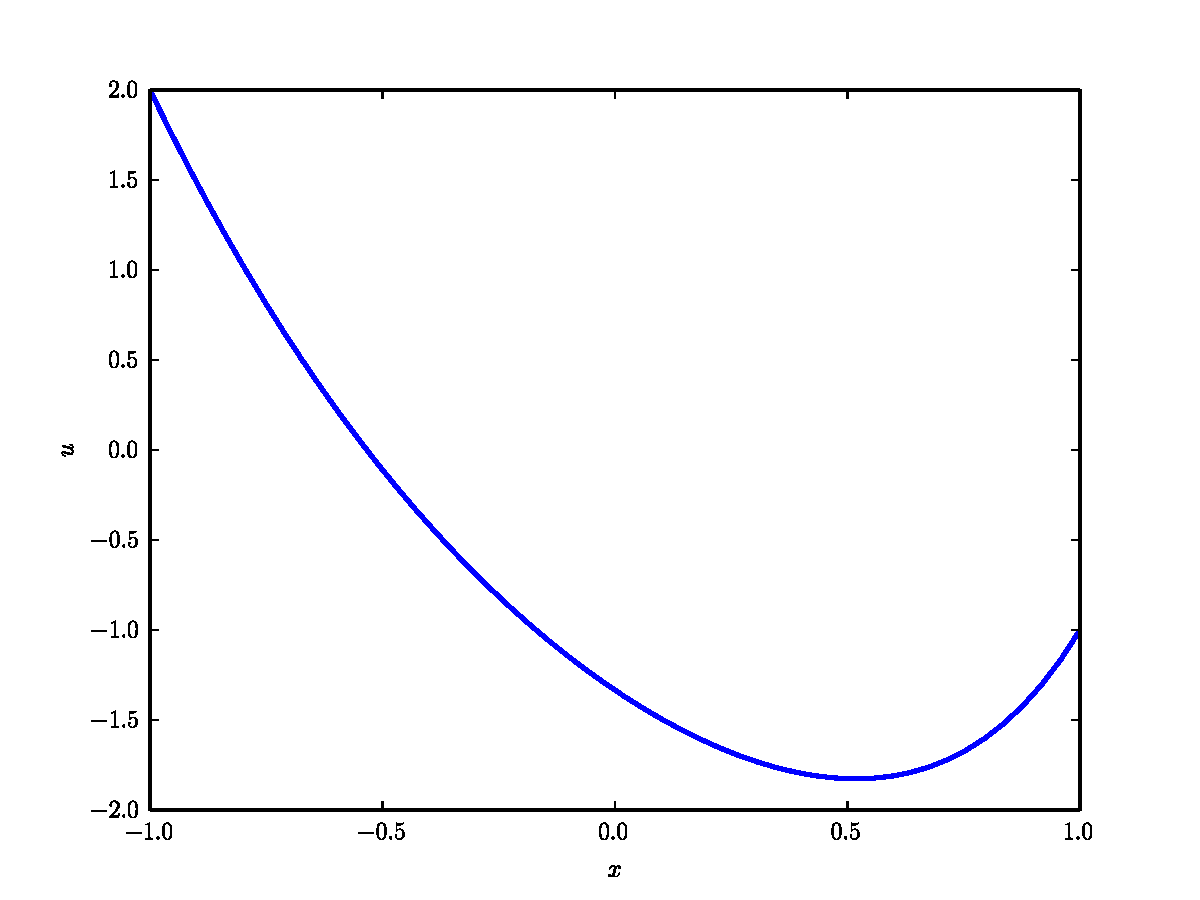
\includegraphics[width=\textwidth]{nonzeroDirichlet.pdf}
\caption{The solution of $u'' + u' = e^{3x}$, subject to the boundary conditions 
$u(-1) = 2$, $u(1) = -1$.}
\label{fig:nonzeroDirichlet}
\end{figure}

\begin{problem}
Use the pseudospectral method to solve the boundary value problem 
\begin{align*}
u'' + u' &= e^{3x}, \\
u(-1) &= 2, \\
u(1) &= -1.
\end{align*}
Check that your numerical solution is converging.
How many subintervals are required to find the solution correct to three decimal places?
See Figure \ref{fig:nonzeroDirichlet}.
	
Hint: Reduce the problem to one with zero Dirichlet conditions by letting $u = U+G$, where $G$ is a (simple) function satisfying the boundary conditions.
\end{problem}

\begin{comment}
\section*{The Method of Weighted Residuals}
We may write our differential/integral equation in operator notation as 
\[(Lu)(x) = f(x), \quad x \in \Omega\]
where $u$ belongs to some infinite-dimensional function space $V.$
We seek for an approximation $u_N$ to the solution $u$.
Our approximation $u_N$ will come from a finite-dimensional function space $S_N$ called the trial space.
Here we use $N$ to denote the dimension of $S_N \subset V$. 
The space $S_N$ can be described by a basis $\{\phi_1(x), \ldots, \phi_N(x)\}$.
Then an approximation $u_N \in S_N$ has the form 
\[u_N = \sum_{j=1}^N \gamma_j \phi_j\]

We can then define an operator $\mathcal{R}$ on the trial space $S_N$ by 
\[\mathcal{R}u_N(x) = Lu_N(x) - f(x)\] 
$\mathcal{R}u_N$ is called the residual or the error of the trial function $u_N$.
Note that the residual of the true solution $u$ is zero.
The method of weighted residuals is a family of methods that determine the coefficients $\gamma_j$ of the approximate solution $u_N$ by forcing the residual $\mathcal{R}u_N$ to be zero in some weighted average over $\Omega$.
In other words, given some collection of weight/test functions $\{w_i\}_{i=1}^M$, we require that 
\begin{align}
\int_{\Omega}\mathcal{R}u_N(x) w_i(x)\, dx &= 0, \quad \text{ for } i = 1, \ldots M
\label{eqn:Spectral1_weightedaverage}
\end{align}

After doing the integration described by (\ref{eqn:Spectral1_weightedaverage}), we obtain a system of algebraic equations that may be used to determine the coefficients $\gamma_i$.
Different choices of the trial space $S_N$ and the weight/test functions $w_i(x)$ result in different methods. 

We obtain the pseudospectral method (or collocation method) by choosing a collection of points $\{x_i\}_{i=1}^M$ in our space $\Omega$ called collocation points.
The weight functions $w_i(x)$ are then given by $w_i(x) = \delta(x-x_i); $ that is, $w_i$ is the Dirac delta function centered at $x_i$.
Then the equations \ref{eqn:Spectral1_weightedaverage} are given by 
\begin{align*}
	\int_{\Omega} \mathcal{R}u_N w_i(x) \, dx &= 0,\\
	\int_{\Omega} \mathcal{R}u_N \delta(x-x_i) \, dx &= 0, \\
	\mathcal{R}u_N(x_i) &= 0 \quad \text{ for } i = 1, \ldots, M
\end{align*}
Thus the pseudospectral method requires the residual of the approximate solution to be exactly zero at the collocation points.
Alternatively, the approximate solution satisfies the differential equation exactly at the collocation points. 
\end{comment}